%%%%%%%%%%%%%%%%%%%%%%%%%%%%%%%%%%%%%%%%%%%
%
% From a template maintained at https://github.com/jamesrobertlloyd/cbl-tikz-poster
%
% Code near the top should be fairly standard and not need to be changed
%  - except for the document class
% Code lower down is more likely to be customised
%
%%%%%%%%%%%%%%%%%%%%%%%%%%%%%%%%%%%%%%%%%%%

%%%%%%%%%%%%%%%%%%%%%%%%%%%%%%%%%%%%%%%%%%%
%
% Document class
%
% Change this if you want a different size / orientation poster etc
%
%%%%%%%%%%%%%%%%%%%%%%%%%%%%%%%%%%%%%%%%%%%

\documentclass[landscape,a0b,final,a4resizeable]{a0poster}
%\documentclass[portrait,a0b,final,a4resizeable]{a0poster}

%%%%%%%%%%%%%%%%%%%%%%%%%%%%%%%%%%%%%%%%%%%
%
% 'Basic' packages
%
% TODO - Almost certainly some are unnecessary - feel free to remove nonstandard
% packages if you think it is a good idea not to always have them
%
%%%%%%%%%%%%%%%%%%%%%%%%%%%%%%%%%%%%%%%%%%%

\usepackage{multicol}
\usepackage{color}
\usepackage{shadow}
\usepackage{morefloats}
\usepackage{cite}
\usepackage[pdftex]{graphicx}
\usepackage{rotating}
\usepackage{amsmath, amsthm, amssymb, bm}
\usepackage{array}
\usepackage{nth}
\usepackage[square,numbers]{natbib}
\usepackage{booktabs}
\usepackage[pdf]{graphviz}

%%%%%%%%%%%%%%%%%%%%%%%%%%%%%%%%%%%%%%%%%%%
%
% TIKZ packages and common definitions
%
% Add extra things as per your tikz needs
%
%%%%%%%%%%%%%%%%%%%%%%%%%%%%%%%%%%%%%%%%%%%

\usepackage{common/picins}
\usepackage{tikz}
\usetikzlibrary{shapes.geometric,arrows,chains,matrix,positioning,scopes,calc}
\tikzstyle{mybox} = [draw=white, rectangle]

%%%%%%%%%%%%%%%%%%%%%%%%%%%%%%%%%%%%%%%%%%%
%
% myfig
%
% \myfig - replacement for \figure
% necessary, since in multicol-environment 
% \figure won't work        
%                 
%%%%%%%%%%%%%%%%%%%%%%%%%%%%%%%%%%%%%%%%%%%

\newcommand{\myfig}[3][0]{
\begin{center}
  \vspace{1.5cm}
  \includegraphics[width=#3\hsize,angle=#1]{#2}
  \nobreak\medskip
\end{center}}

%%%%%%%%%%%%%%%%%%%%%%%%%%%%%%%%%%%%%%%%%%%
%
% mycaption                
%
% \mycaption - replacement for \caption
% necessary, since in multicol-environment \figure and
% therefore \caption won't work
%
%%%%%%%%%%%%%%%%%%%%%%%%%%%%%%%%%%%%%%%%%%%

%\newcounter{figure}
% \setcounter{figure}{1}
\newcommand{\mycaption}[1]{
  \begin{quote}
    \centering
    \textit{#1}
  \end{quote}
  \stepcounter{figure}
}

%%%%%%%%%%%%%%%%%%%%%%%%%%%%%%%%%%%%%%%%%%%
%
% Some standard colours
%
%%%%%%%%%%%%%%%%%%%%%%%%%%%%%%%%%%%%%%%%%%%

\definecolor{camlightblue}{rgb}{0.601 , 0.8, 1}
\definecolor{camdarkblue}{rgb}{0, 0.203, 0.402}
\definecolor{camred}{rgb}{1, 0.203, 0}
\definecolor{camyellow}{rgb}{1, 0.8, 0}
\definecolor{lightblue}{rgb}{0, 0, 0.80}
\definecolor{white}{rgb}{1, 1, 1}
\definecolor{whiteblue}{rgb}{0.80, 0.80, 1}

%%%%%%%%%%%%%%%%%%%%%%%%%%%%%%%%%%%%%%%%%%%
%
% Some look and feel definitions
%
%%%%%%%%%%%%%%%%%%%%%%%%%%%%%%%%%%%%%%%%%%%

\setlength{\columnsep}{0.03\textwidth}
\setlength{\columnseprule}{0.0018\textwidth}
\setlength{\parindent}{0.0cm}

%%%%%%%%%%%%%%%%%%%%%%%%%%%%%%%%%%%%%%%%%%%
%
% \mysection - replacement for \section*
% 
% Puts a pretty box around some text
% TODO - any other thoughts for what this box should look like
%
%%%%%%%%%%%%%%%%%%%%%%%%%%%%%%%%%%%%%%%%%%%

\tikzstyle{mysection} = [rectangle, 
									draw=none, 
									shade, 
									outer color=camlightblue!30,
									inner color=camlightblue!30,
									text width=0.965\columnwidth,
									text centered,
									rounded corners=20pt,
									minimum height=0.11\columnwidth]

\newcommand{\mysection}[1]
{
\begin{center}
  \begin{tikzpicture}
    \node[mysection] {\sffamily\bfseries\LARGE#1};
  \end{tikzpicture}
\end{center}
}

%%%%%%%%%%%%%%%%%%%%%%%%%%%%%%%%%%%%%%%%%%%
%
% Set the font
%
% TODO - Not sure what a canonical choice is - feel free to modify
%
%%%%%%%%%%%%%%%%%%%%%%%%%%%%%%%%%%%%%%%%%%%

\renewcommand{\familydefault}{cmss}
\sffamily

%%%%%%%%%%%%%%%%%%%%%%%%%%%%%%%%%%%%%%%%%%%
%
% Poster environment
%
% Centres everything and can be used to define the width of the content
%
%%%%%%%%%%%%%%%%%%%%%%%%%%%%%%%%%%%%%%%%%%%

\newenvironment{poster}{
  \begin{center}
  \begin{minipage}[c]{0.96\textwidth}
}{
  \end{minipage} 
  \end{center}
}

%%%%%%%%%%%%%%%%%%%%%%%%%%%%%%%%%%%%%%%%%%%
%
% This is probably a good place to put content specific packages and definitions
%
%%%%%%%%%%%%%%%%%%%%%%%%%%%%%%%%%%%%%%%%%%%

\newtheorem{thm}{Theorem}%[section]
\newtheorem{lem}[thm]{Lemma}
\newtheorem{prop}[thm]{Proposition}
\newtheorem{cor}[thm]{Corollary}

\newtheorem*{theorem*}{Theorem}

\theoremstyle{definition}
\newtheorem*{definition*}{Definition}
\newtheorem{definition}[thm]{Definition}%[section]
\newtheorem{conj}{Conjecture}[section]
\newtheorem{exmp}{Example}[section]
\newtheorem{rem}[thm]{Remark}

\theoremstyle{remark}
%\newtheorem{rem}{Remark}
\newtheorem{note}{Note}
\newtheorem{case}{Case}

\newcommand{\eqd}{\overset{\,_{\!d}}{=}}
\newcommand{\defn}[1]{\emph{#1}}

\newcommand{\Law}{\mathcal{L}}

\def\given{\,|\,}

\def\SGinf{\mathbb{S}_{\infty}}

\newcommand{\NonNegInts}{\mathbb{Z}_+}
\newcommand{\Nats}{\mathbb{N}}
\newcommand{\Rationals}{\mathbb{Q}}
\newcommand{\Reals}{\mathbb{R}}

\newcommand{\as}{\textrm{a.s.}}

\def\[#1\]{\begin{align}#1\end{align}}
\newcommand{\defas}{:=}

\newcommand{\Normal}{\mathcal{N}}
\newcommand{\dist}{\ \sim\ }

\newcommand{\kernel}{\kappa}
\newcommand{\kernelmatrix}{K}
\newcommand{\scalefactor}{s}
\newcommand{\lengthscale}{\ell}
\newcommand{\targets}{T}
\newcommand{\noise}{\sigma_\targets}
\newcommand{\pseudopoints}{\eta}
\newcommand{\inputpoints}{\xi}
\newcommand{\covhyppar}{\psi}
\newcommand{\logistic}{\phi}

\newcommand{\CompOrder}{\mathcal{O}}
\def\graphspace{\mathbf{G}}
\def\Uniform{\mbox{\rm Uniform}}
\def\Bernoulli{\mbox{\rm Bernoulli}}
\def\ie{i.e.,\ }
\def\eg{e.g.,\ }
\def\iid{i.i.d.\ }
\def\simiid{\sim_{\mbox{\tiny iid}}}
\def\simind{\sim_{\mbox{\tiny ind}}}
\def\eqdist{\stackrel{\mbox{\tiny d}}{=}}
\def\ahfunction{\theta}       
\def\AHfunction{\Theta}           % A-H random function
\def\AHvar{U}                     % A-H uniform variables
\def\AHvaralt{V}                  % A-H uniform variables - for bipartite data
\def\larray{W}                    % latent array sampled with A-H
%\def\latentspace{\mathbf{W}}      % range of entries
\def\latentspace{\mathcal{W}}      % range of entries
\def\darray{X}                    % data array
%\def\dataspace{\mathbf{X}}        % sample space
\def\dataspace{\mathcal{X}}        % sample space
\def\cfspace{\mathbf{C}}          % space of continuous functions
%\def\GP{\mbox{\mathcal{GP}}}
\def\GP{\mathcal{GP}}
\def\likelihood{P}
\def\CovData{C}
\def\CovDataAlt{D}

\def\newarrow{\mbox{\begin{tikzpicture}
             \useasboundingbox{(-3pt,-4.5pt) rectangle (19pt,1pt)};
             \draw[->] (0,-0.07)--(17pt,-0.07);\end{tikzpicture}}}

%%%%%%%%%%%%%%%%%%%%%%%%%%%%%%%%%%%%%%%%%%%
%
% The document environment starts here
%
%%%%%%%%%%%%%%%%%%%%%%%%%%%%%%%%%%%%%%%%%%%

\begin{document}

%%%%%%%%%%%%%%%%%%%%%%%%%%%%%%%%%%%%%%%%%%%
%
% Begin the poster environment - centres things and potentially changes the width
%
%%%%%%%%%%%%%%%%%%%%%%%%%%%%%%%%%%%%%%%%%%%

\begin{poster}

  %%%%%%%%%%%%%%%%%%%%%%%%%%%%%%%%%%%%%%%%%%%
  %
  % Potentially add some space at the top of the poster
  %
  %%%%%%%%%%%%%%%%%%%%%%%%%%%%%%%%%%%%%%%%%%%

  \vspace{0\baselineskip}

  %%%%%%%%%%%%%%%%%%%%%%%%%%%%%%%%%%%%%%%%%%%
  %
  % Draw the header as a TIKZ picture
  %
  % Using TIKZ to allow for easy alignment
  %
  %%%%%%%%%%%%%%%%%%%%%%%%%%%%%%%%%%%%%%%%%%%

  \begin{center}
    \begin{tikzpicture}[x=0.5\textwidth]
      % Dummy nodes at edges for spacing
      % TODO - a better way?
      \node at (+1, 0) {};
      \node at (-1, 0) {};
      % Set the size of the badges
      \def \badgeheight {0.08\textwidth}
      % Title text
      \node[inner sep=0,text width=0.75\textwidth,text centered,font=\Huge] (Title) at (0,0)
      {
      {\sffamily \Huge \textbf{Personalized Recipe Recommendation Using Heterogeneous Graphs}}\\
      {\huge\sffamily
      Nicholas B. DeGroot
      }\\
      \vspace{-0.3\baselineskip}
      {\large\sffamily
        Halıcıoğlu Data Science Institute, UC San Diego
      }
      };
      % UCSD badge
      \node [mybox] (UCSD Badge) at (-0.9, 0) {
        
\includegraphics[height=\badgeheight]{badges/ucsdseal.png}
      };
      % TigerGraph badge
      \node [mybox] (TigerGraph Badge) at (0.9, 0) {
        
\includegraphics[height=\badgeheight]{badges/tigergraph.png}
      };
    \end{tikzpicture}
  \end{center}
  %%%%%%%%%%%%%%%%%%%%%%%%%%%%%%%%%%%%%%%%%%%
  %
  % Spacing between title and main body
  %
  %%%%%%%%%%%%%%%%%%%%%%%%%%%%%%%%%%%%%%%%%%%

  \vspace{1\baselineskip}

  %%%%%%%%%%%%%%%%%%%%%%%%%%%%%%%%%%%%%%%%%%%
  %
  % Columns environment
  %
  %%%%%%%%%%%%%%%%%%%%%%%%%%%%%%%%%%%%%%%%%%%

  \begin{multicols}{3}

    %%%%%%%%%%%%%%%%%%%%%%%%%%%%%%%%%%%%%%%%%%%
    %
    % Start of content
    %
    %%%%%%%%%%%%%%%%%%%%%%%%%%%%%%%%%%%%%%%%%%%

    \large

    \mysection{Abstract}

    \begin{itemize}
      \item We propose a system that can automate the process of meal planning and grocery shopping.
      \item TigerGraph is used to store and query heterogeneous graph data, which is then used to generate personalized recipe recommendations.
      \item We experiment with several ways to model heterogeneous graph data using the LightGCN architecture, finding that pure latent features perform best.
    \end{itemize}

    \vspace{\baselineskip}
    \mysection{Motivation}

    \begin{center}
      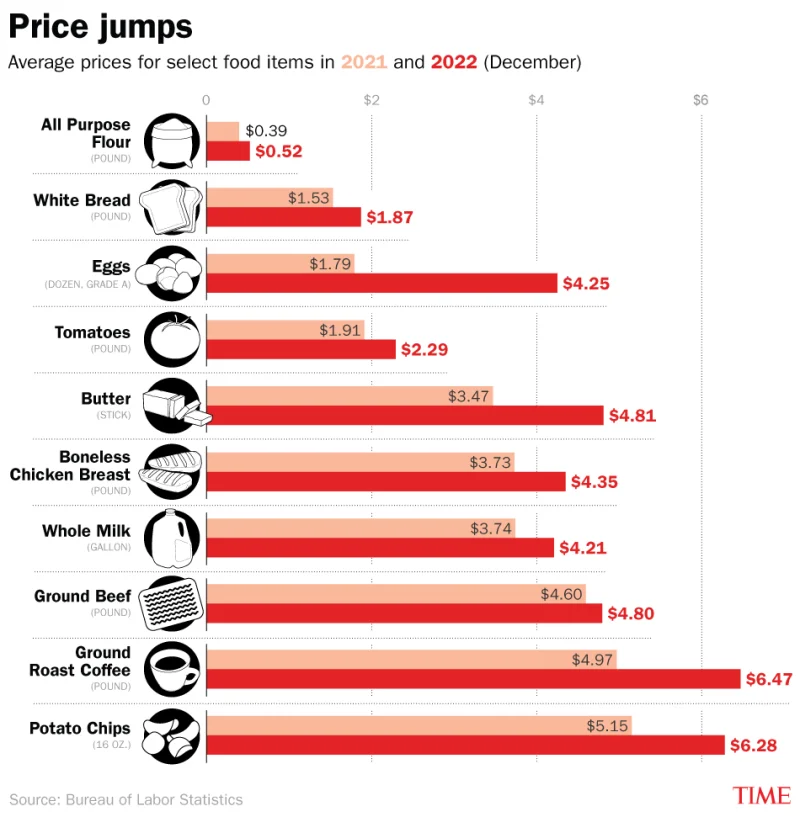
\includegraphics[height=9\baselineskip]{figures/food-inflation.png}
      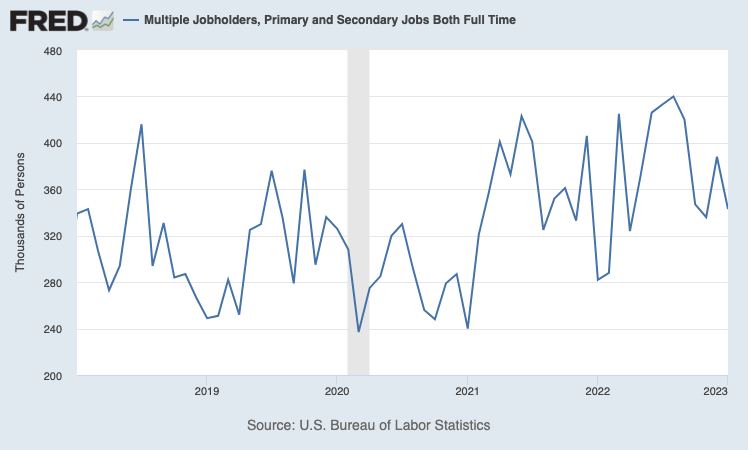
\includegraphics[height=9\baselineskip]{figures/two-jobs.png}
      \mycaption{Left: Increase in Average Price of Groceries\\Right: Increase in Multiple Full Time Job Holders}
    \end{center}

    This project was born from some recent insights in the economy:
    \begin{itemize}
      \item The average cost of groceries for a household has risen by 13.5\% over the last year.
      \item Roughly 388,000 Americans are currently working more than two \textbf{full time} jobs (nearly 5\% of the workforce).
    \end{itemize}

    In essence, people can't afford to eat out due to budget constraints, but can't afford to eat at home due to time constraints. To this end, we propose a system that can automate the process of meal planning and grocery shopping. By automatically generating meal plans custom tailored to the users taste preferences, users save the time previously spent planning meals and the money previously spent eating out.

    \vspace{\baselineskip}
    \mysection{Data Modeling}

    The data for this project was sourced from \verb|food.com| in the form of recipes and reviews. After downloading and extracting the data, we modeled and stored the data in a graph database using the TigerGraph platform. Using TigerGraph allowed us to easily model the data as a heterogeneous graph, which is a graph where nodes can be stored as different types. The graph database schema is shown below.

    % https://mermaid.live/edit#pako:eNp1kdFLwzAQxv-VkCeFDpzFVQs-CCIIY8Kcb4FxS25dsElKchHG6P9u2lqcWu8p_L7vctx3Jy6dQl5yWUMIjxoqD0ZYlkppj5K0s2y9FHZgvYu9BfSnAXR1cclW7J5d32RXxWLA7bl9jVI3yCY68nm2yIvx866eVxtmtI2E4Se020DYnMGn5cvDhkmondf4h5MjqLd7oG2jPn6LIVbgJwWndDRTSuMdobaTTUDRA6H6b5wEv3OHo-pM4dvQjnt3cbLZbMyp7PdNZm0rIWwXVDG_zfLijmfcoDegVTpYH6fgdECDgpfpqcC_Cy5sm3wQyb0ereQl-YgZj41K07_uy8s91AHbT4Uuluo
    \vspace{\baselineskip}

    \begin{tabular}{cc}
      \begin{minipage}[c]{0.4\columnwidth}
        \begin{centering}
          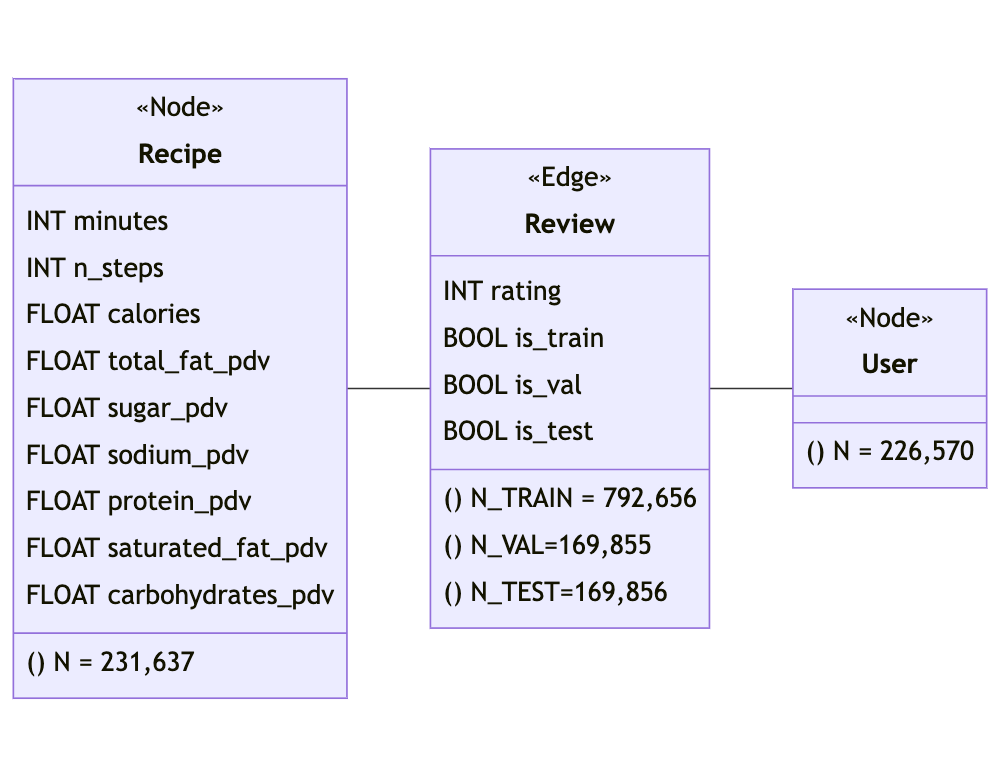
\includegraphics[width=\linewidth]{figures/schema.png}
        \end{centering}
      \end{minipage}
       &
      \begin{minipage}[c]{0.6\columnwidth}

        For the purpose of this project, we exported the data from TigerGraph in CSV format to our local machine. This was then imported using standard python libraries.

      \end{minipage}
    \end{tabular}

    \newpage
    \mysection{Collaborative Filtering}

    Our first non-trivial attempt at recommending recipes to users was to use a collaborative filtering model. Collaborative filtering is a classical algorithm that recommends items to users under the assumption that users with similar tastes will like similar items.

    \vspace{\baselineskip}

    The model works by first computing a similarity score between users. We chose to use the pearson correlation coefficient as our similarity metric, due to its ability to handle non-centered ratings. The model then ranks each recipe based on the the similarity of users who've rated the recipe and the rating they gave it.

    $$
      \text{Recipe Score}
      = \sum_{u'}
      \text{Similarity}(u, u') \cdot
      (\text{Rating}(u', r) - \mu_{u'})
    $$

    One huge benefit of this model is that it can be run on-demand inside TigerGraph using GSQL. This allows for easy integration with systems that need to make recommendations in real-time.

    \vspace{\baselineskip}
    \mysection{Graph Neural Networks}

    Our second model attempted to use a graph neural network to recommend recipes to users. Graph neural networks are a relatively new class of neural network that are designed to make use of the structure of a graph.

    \vspace{\baselineskip}

    Our first attempt at using a graph neural network was to build off the \textbf{LightGCN} architecture. LightGCN is a graph neural network built specifically for recommendation tasks. It works by taking one learned layer (the node embeddings), and propagating it through the graph using a normalized sum.

    \begin{center}
      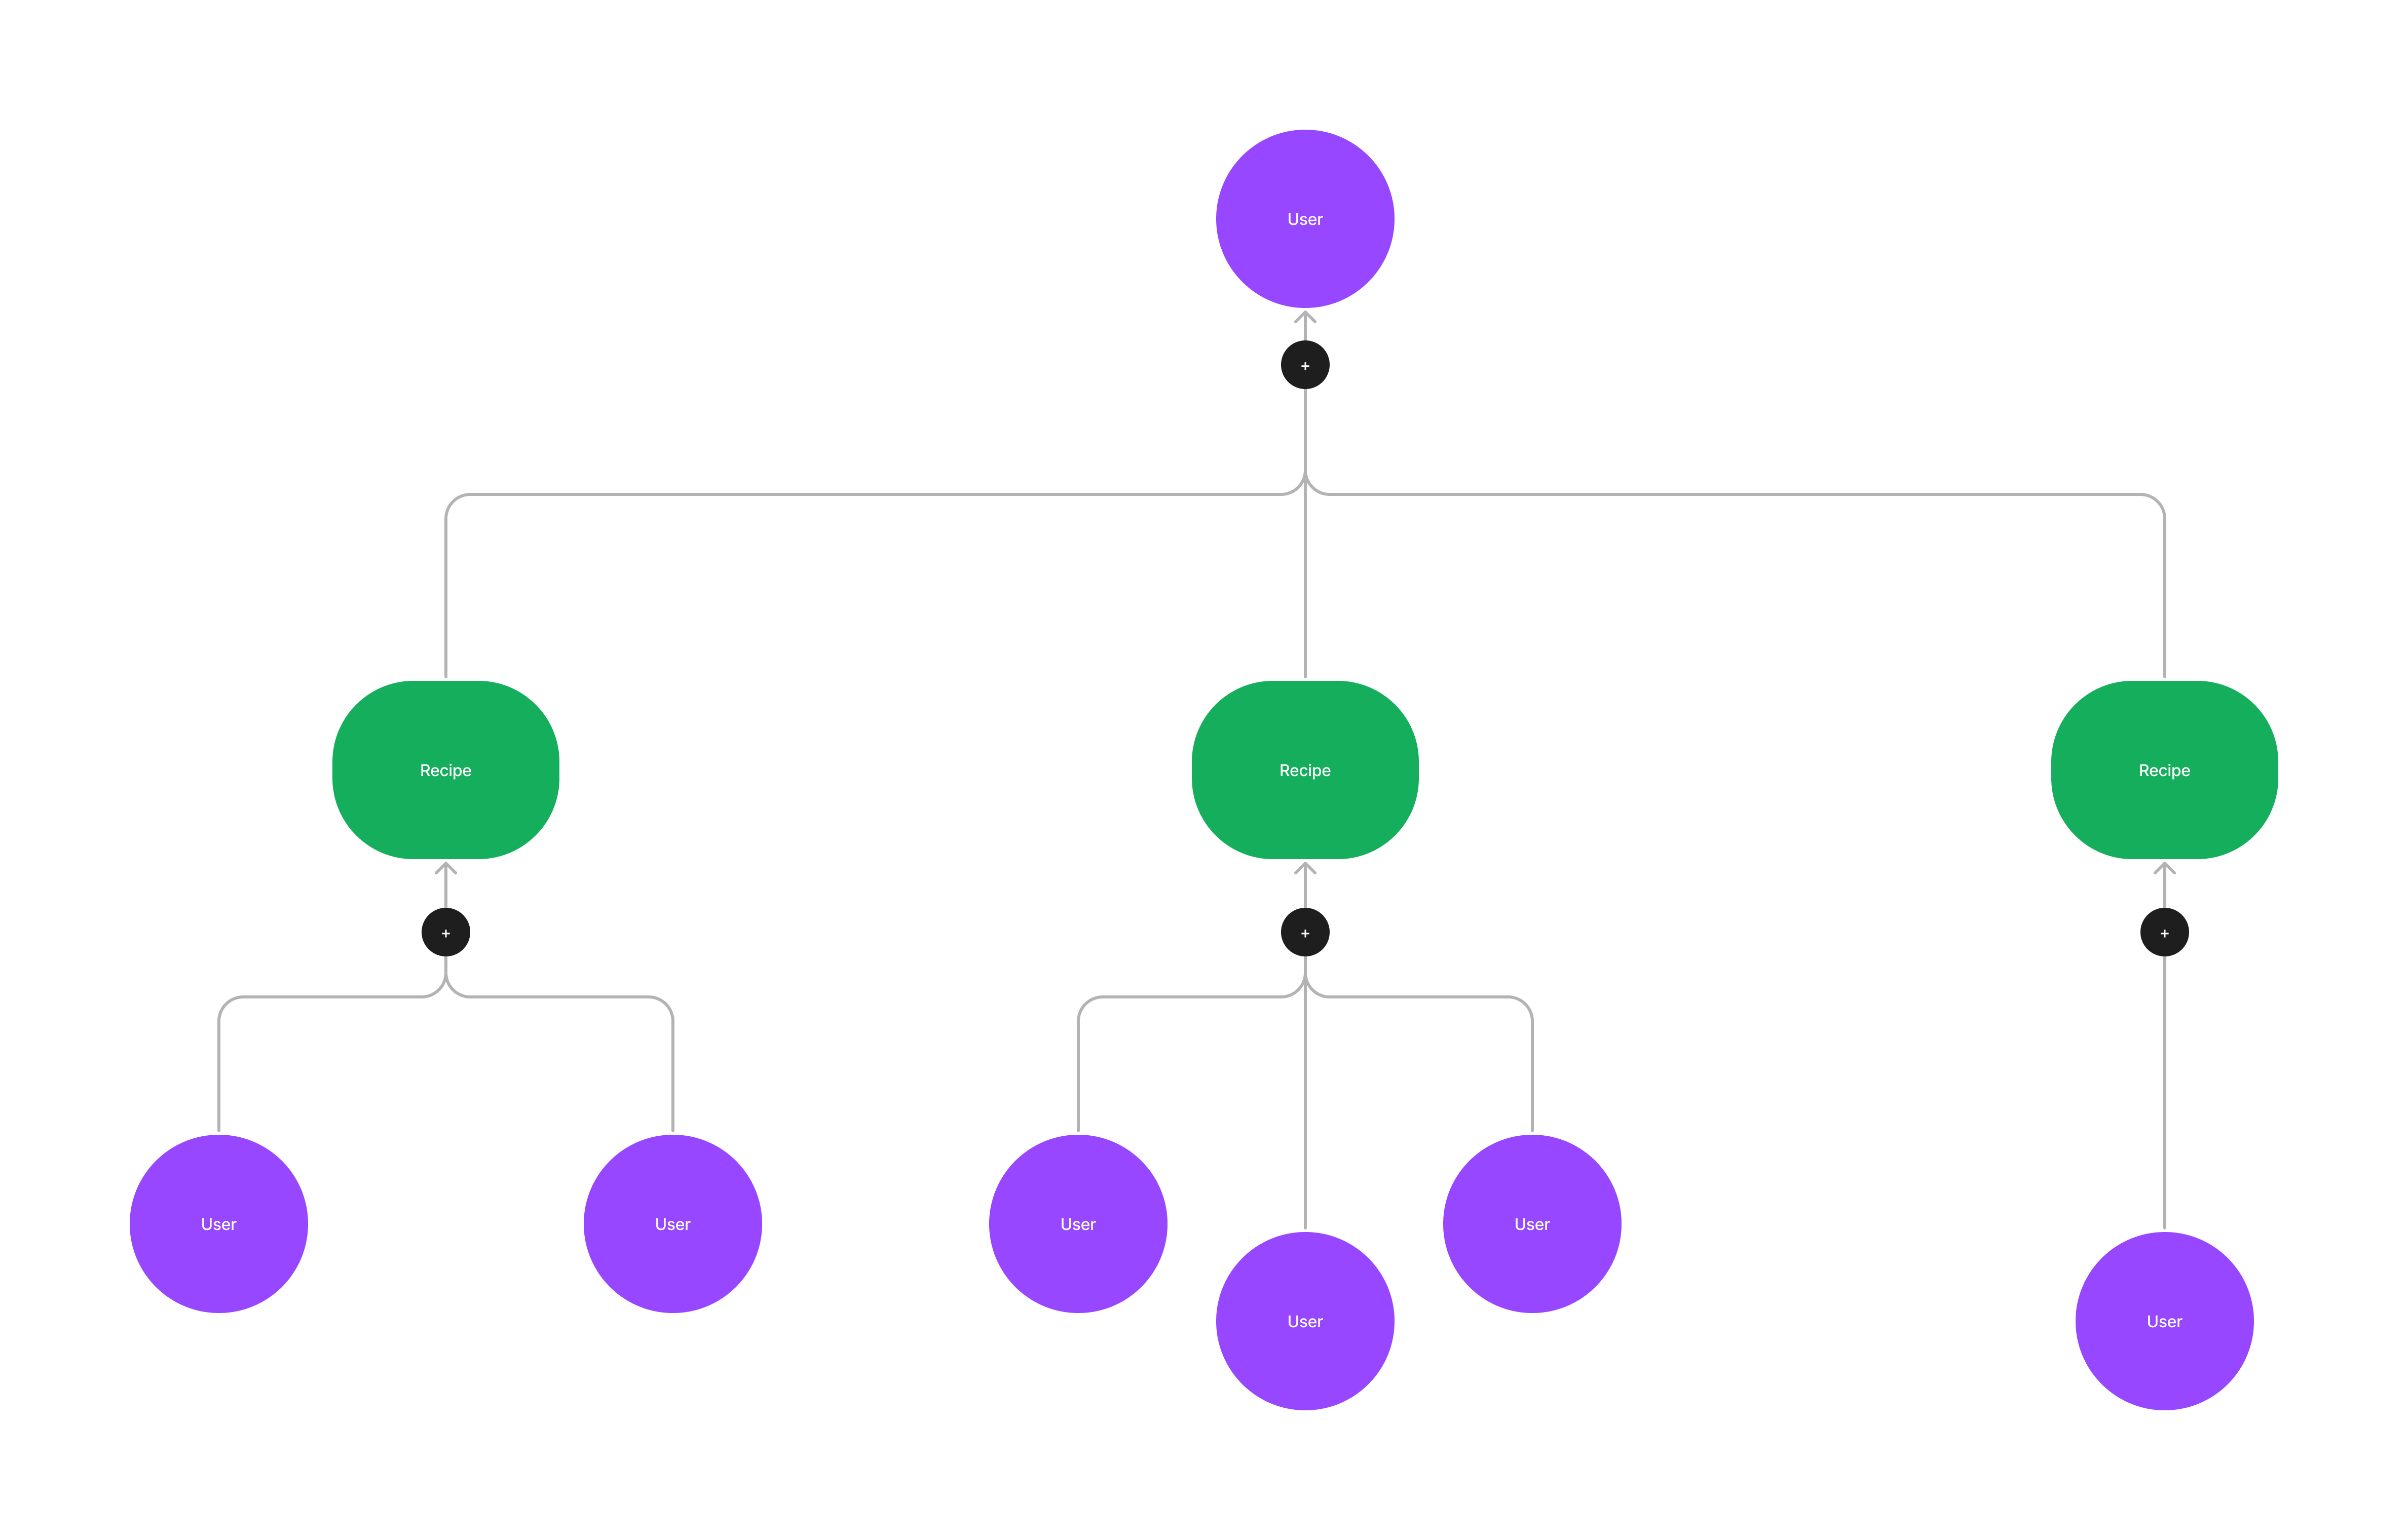
\includegraphics[width=0.4\columnwidth]{figures/gcn.png}
    \end{center}

    The main problem with using the LightGCN architecture is that it is not designed to handle heterogeneous graphs. For the model embeddings to be propagated, the graph must have the same dimensionality for all nodes. To solve this, we experimented with three different methods of handling the heterogeneous graph:

    \vspace{\baselineskip}

    \begin{itemize}
      \item \textbf{Latent Features}: The simplest method is to discard any node information and learn embeddings through latent features. This method is analogous to the original implementation.
      \item \textbf{Opposite Embedding}: The second method is to learn embeddings for the (normalized) opposite node's features. This method can be thought of as learning the node's affinity for those specific features.
      \item \textbf{Combination}: The third method is to combine the two previous methods.
    \end{itemize}

    \vspace{\baselineskip}

    For each method, we trained a model for 2000 epochs on the train set using bayesian personalized ranking loss. The best model was chosen based on precision@10 against a pre-split evaluation set.

    \newpage
    \mysection{Comparison of Methods}

    \begin{center}
      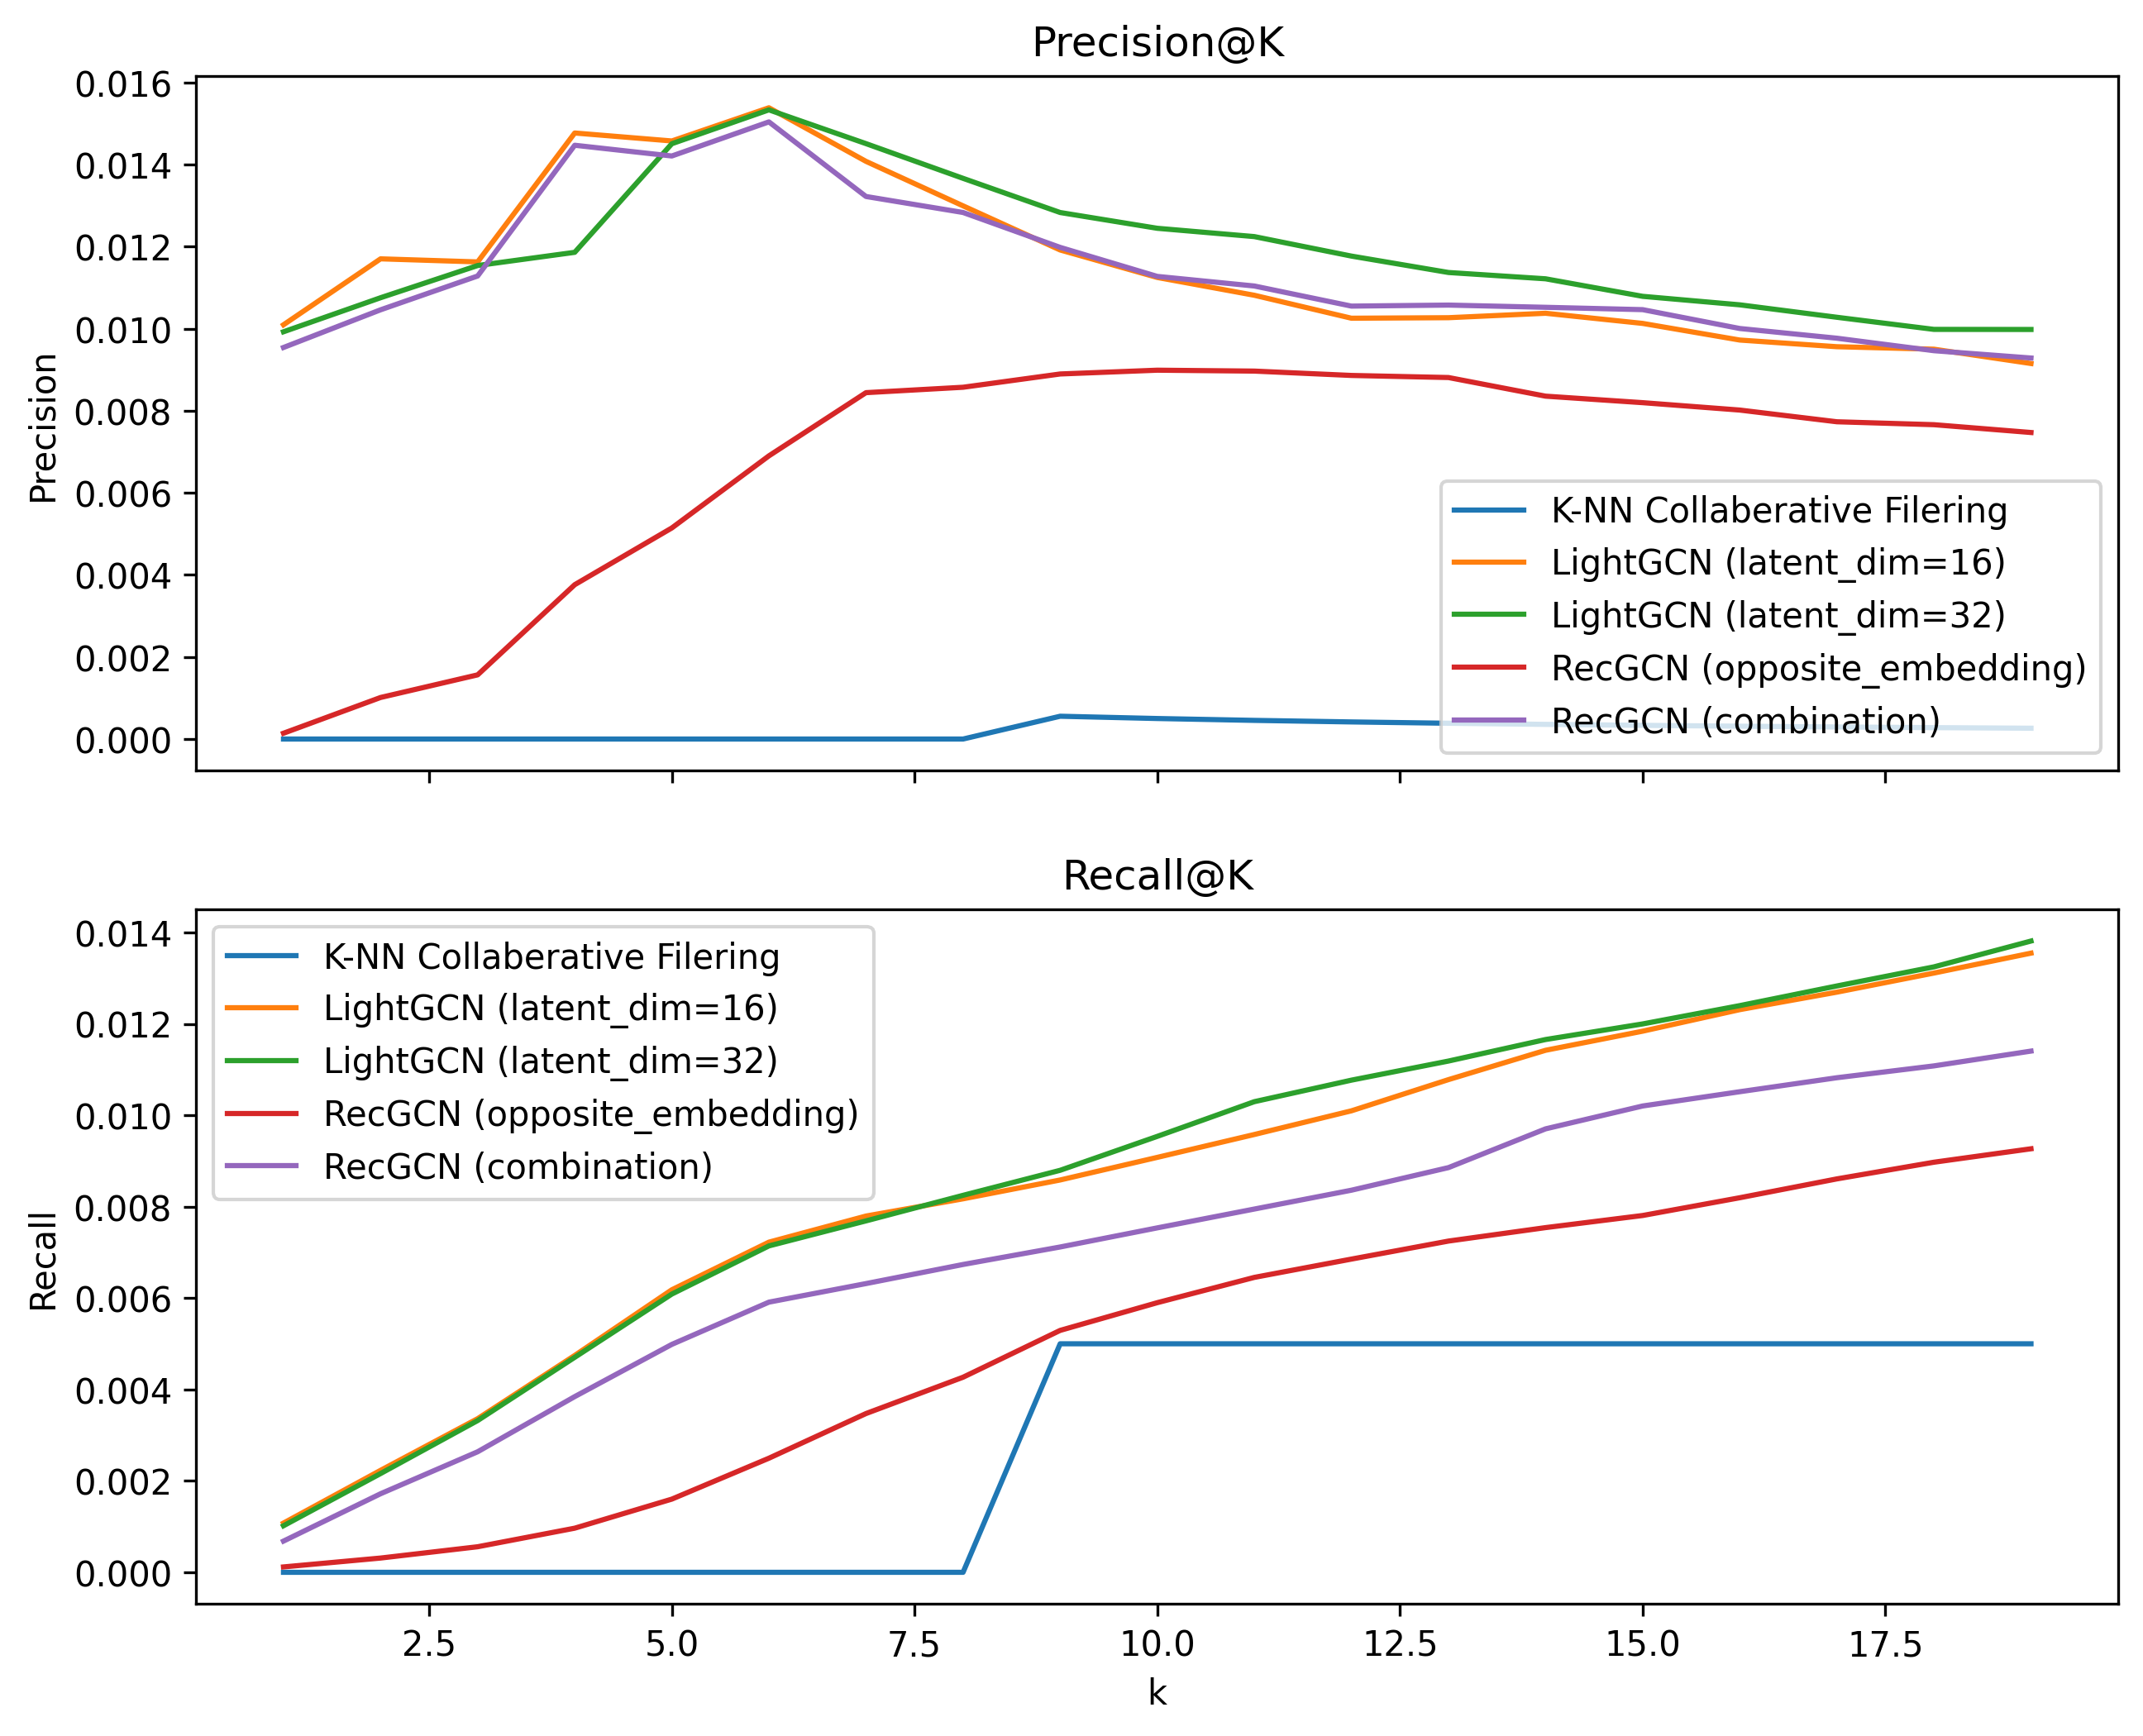
\includegraphics[width=0.4\columnwidth]{figures/model_eval.png}
      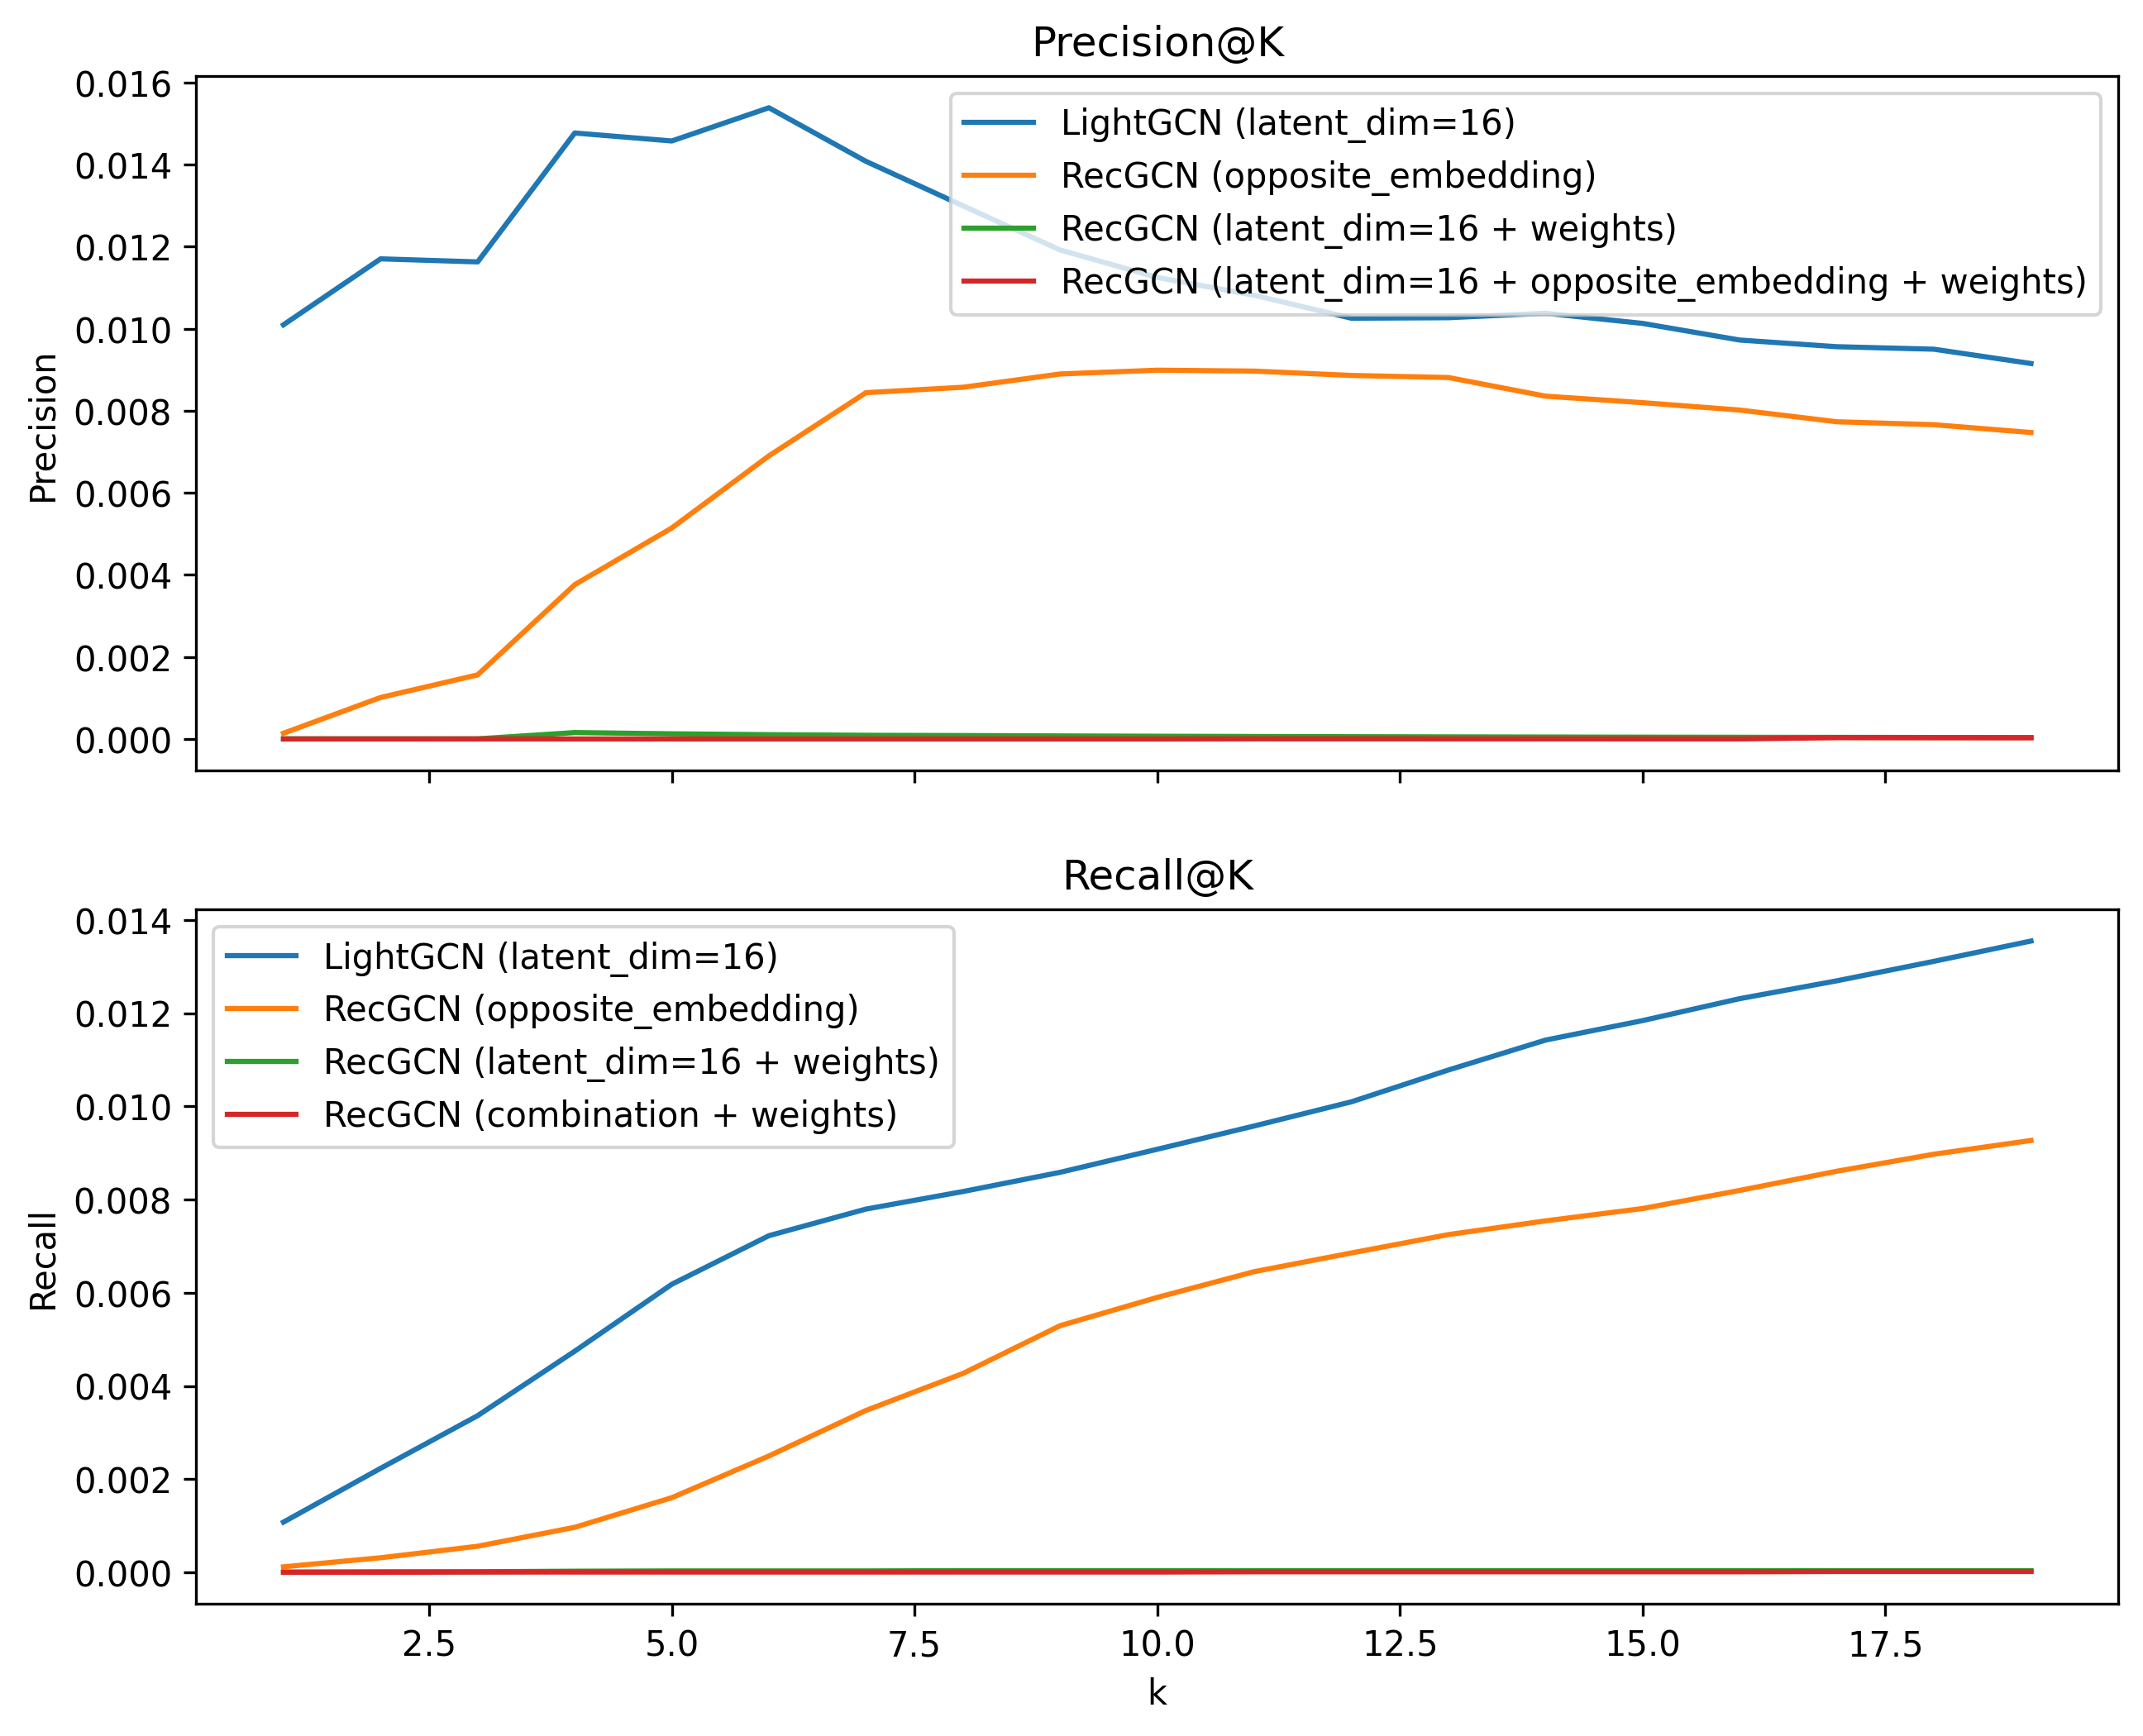
\includegraphics[width=0.4\columnwidth]{figures/flag_eval.png}
    \end{center}

    \begin{itemize}
      \item \textbf{Collaborative Filtering}: Could not accurately recommend recipes to users. A closer look revealed that the model was heavily reliant on the test items appearing in the training history, which was wasn't the case for most of the pre-split set.
      \item \textbf{GCN w/ Latent Features}: The model was able to recommend recipes to users extremely well, as suggested by the original paper.
      \item \textbf{GCN w/ Opposite Embedding}: The model was not able to recommend recipes to users very well. This may be a result of the smaller number of embedding dimensions.
      \item \textbf{GCN w/ Combination}: This model performed slightly \textit{worse} then just using latent features, suggesting that the LightGCN architecture has a hard time learning non-latent features.
    \end{itemize}

    We additionally experimented with weighting the aggregations by the normalized user rating. Surprisingly, this had a extreme \textit{negative} effect of model performance.


    \vspace{\baselineskip}
    \mysection{Future Work}

    \begin{center}
      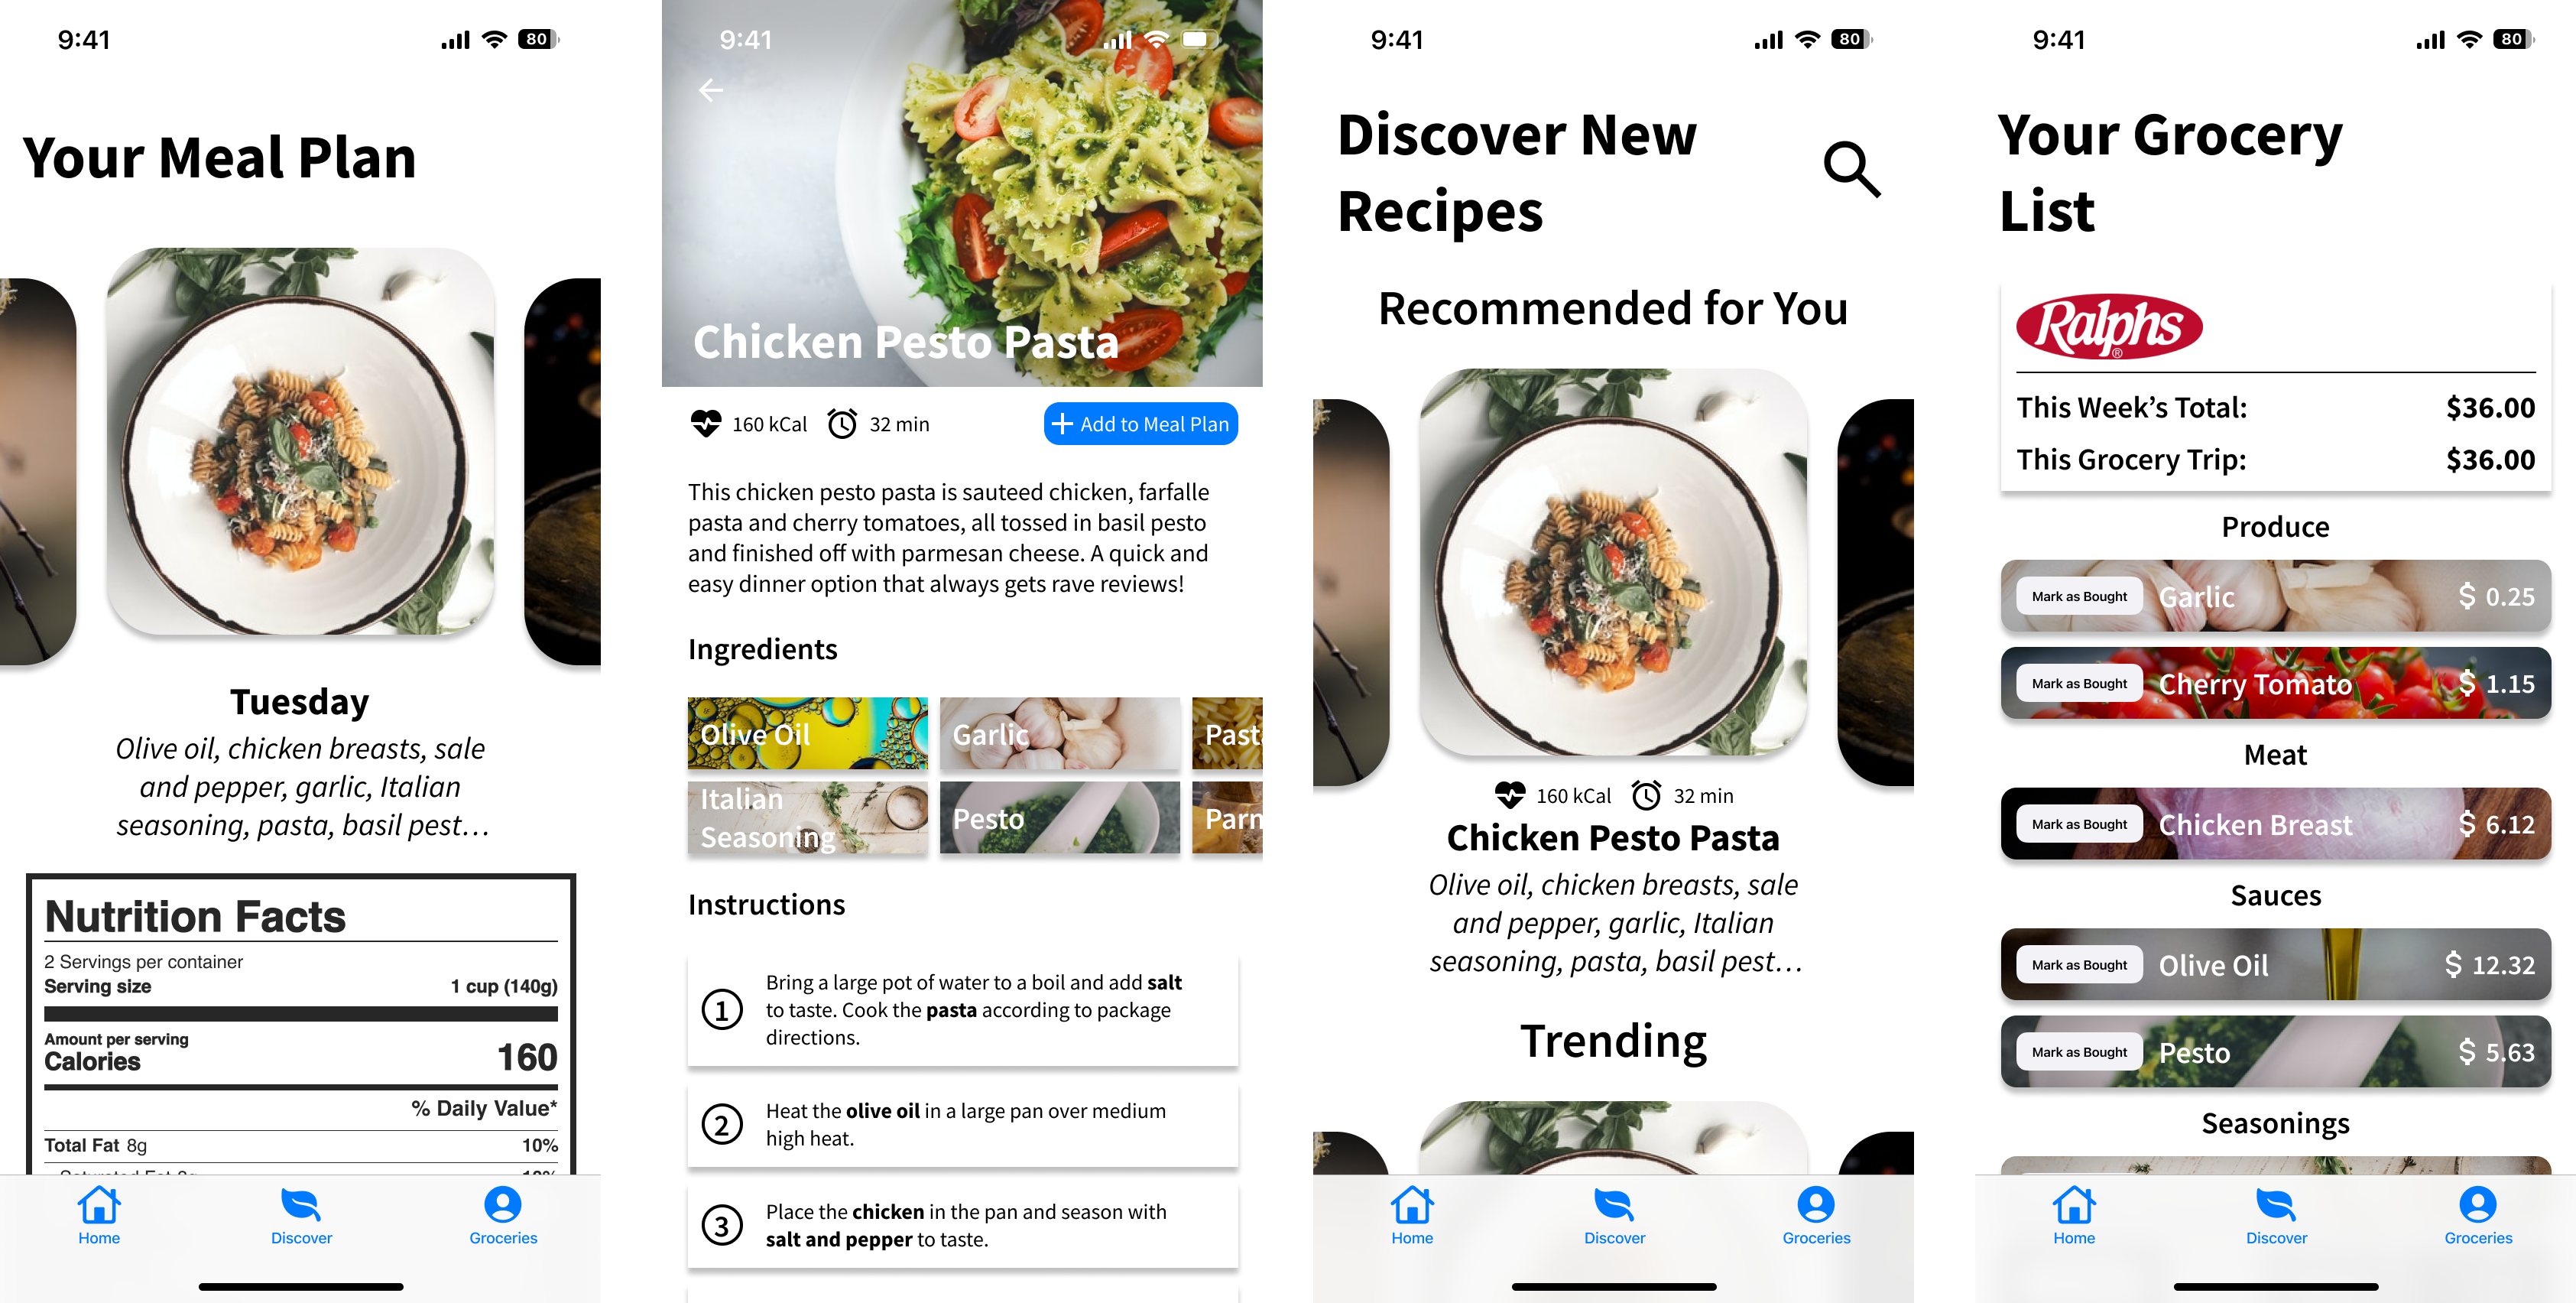
\includegraphics[width=0.4\columnwidth]{figures/ux.png}
      \mycaption{Current UX Mockup}
    \end{center}

    We plan to continue this work in a commercial setting. We believe that this project can be a core component of a full system that helps people save time and money by automating the process of meal planning and grocery shopping.


    \vspace{\baselineskip}
    Future work includes:
    \begin{itemize}
      \item \textbf{User Interface}: Performing a user study to determine the best way to present the recommendations to the user.
      \item \textbf{Software Development}: Developing the core app to be used by the user.
      \item \textbf{Recommendation Improvements}: Experimenting with different models to improve the recommendations.
    \end{itemize}

    \begin{tabular}{cc}
      \begin{minipage}[c]{0.8\columnwidth}

        Website: \texttt{recipe.nickthegroot.com}

        Code: \texttt{github.com/nickthegroot/recipe-recommendation}

        Paper available by scanning the QR code

      \end{minipage}
       &
      \begin{minipage}[c]{0.2\columnwidth}
        \begin{centering}
          
\includegraphics[width=\linewidth]{figures/report_qr.png}
        \end{centering}
      \end{minipage}
    \end{tabular}

  \end{multicols}

\end{poster}

\end{document}
